%\section{Absenteeism group detection algorithms}
The optimal solution to the problem in last section has running time complexity of $O(2^N)$. To reduce the time complexity, in this  section, we propose two approximate optimal solutions, the first is regional approach with time complexity of $O(N^3)$, and the second is subgraph approach, with $O(N^2)$ time complexity.
\subsection{Regional approach}
For further explanation convenience, we define some notations firstly.
\begin{itemize}
  \item Suppose $H(P)=P$, $P$ is called an empty convex polygon, which means all the nodes in $P$ lie in the edges of $H(P)$, and there is no node lies inside of $H(P)$. $P$ is empty does not necessary mean that there is no any city in $\mathcal{T}$ happen to lie inside the convex polygon of $P$, it just mean that $P$ does not contain any node which lies inside $H(P)$. As shown in Figure~\ref{fig:notation}, $P_1=\{c_1,c_2,c_3,c_4\}$ and $P_2=\{c_5, c_6, c_7, c_8, c_9\}$. $P_1$ is empty because $H(P_1)=P_1$. While $P_2$ is not an empty convex polygon, since $H(P_2)=\{c_5, c_6, c_7, c_8\}\neq P_2$.
    \item Suppose $P$ is an empty convex polygon, $g(P)$ is used to represent cities which either lie in the edges of $P$, or inside $H(P)$. We call $g(P)$ is $P$'s domain, and $P$ is the support of $g(P)$. As shown in Figure~\ref{fig:notation}, $P_1$ is an empty convex polygon, and inside $P_1$, there are nodes $c_{11}, c_{12}$, thus $g(P_1)=\{c_1,c_2,c_3,c_4,c_{11},c_{12}\}$.
\end{itemize}

\begin{figure}[t]
	\centering
	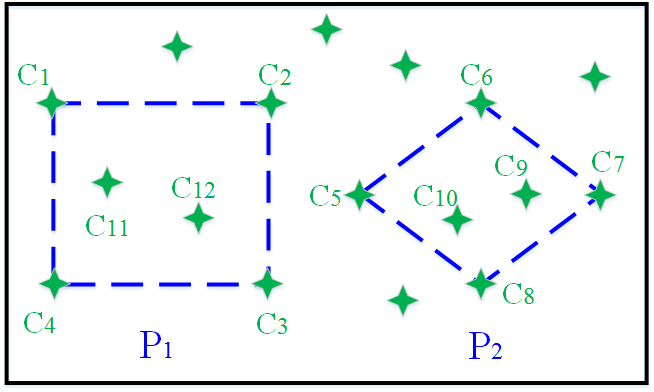
\includegraphics[width=2.2in,height=1.3in]{figures/bruteforce.png}
	\caption{Notation explanation: $P_1=\{c_1,c_2,c_3,c_4\}$, $P_2=\{c_5, c_6, c_7, c_8, c_9\}$. $P_1$ is empty convex polygon, while $P_2$ is not because $H(P_1)=P_1$, and $H(P_2)=\{c_5, c_6, c_7, c_8\}\neq P_2$. $P_1$ is an empty convex polygon, which does not mean there is no any node in $P_1$. Instead, inside $P_1$, there are nodes $c_{11}, c_{12}$, thus $g(P_1)=\{c_1,c_2,c_3,c_4,c_{11},c_{12}\}$.}
	\label{fig:notation}
\end{figure}


\subsubsection{Brute force algorithm}
An obvious brute force algorithm for minimal absenteeism group detection is described in algorithm~\ref{algo:convex_hull}.
\begin{enumerate}
  \item Firstly, it finds out all the empty convex polygons, $\mathcal{P}= \{P_i\}$, $s(P_i)\leq A$, $\forall P_i\in 2^\mathcal{T}$;
  \item Secondly, for each $P_i \in \mathcal{P}$, compute $P_i$'s domain $g(P_i)$, and its group absenteeism score $\Gamma_1(P_i)$;
  \item return the minimal $\Gamma_1(P_i)$, and the corresponding empty convex polygon $P_i$.
\end{enumerate}

\begin{algorithm}[h]
\centering
\captionsetup{font=scriptsize}
\caption{Brute force algorithm}
{\footnotesize \begin{algorithmic}[1]
\STATE {\bf Input:} city set $\mathcal{T}$, score set $\alpha(\mathcal{T})$ and areas upper bound $A$
%, \alpha(\mathcall{T})$: set of sources for location $l$; ${\bf D_l}$: training points; $R_{S_l}$: source-topic relevance dictionary for sources in $S_l$ and points in ${\bf D_l}$; $O_{S_l}$: one-class SVMs for $S_l$; $\epsilon$: discount factor
\STATE {\bf Output:} subset $P$ with lowest absenteeism score, where $P\in 2^{\mathcal{T}}$	
	\FORALL {$K$ from 3 to $N$}
			\FORALL {$P_i$}
			\STATE{enumerate all city set $P_i$, where $|P_i|=K$}
			\IF {$P_i$ is empty}			
					\IF {$s(P_i)\leq A$}
						\STATE{compute $P_i$'s domain $g(P_i)$}
						\STATE{compute group absenteeism score $\Gamma_1(P_i)$}
					\ENDIF
			\ENDIF
	\ENDFOR	
	\ENDFOR	
\RETURN $\min\Gamma(g(P_i))$, and $P_i$
\end{algorithmic}}
\label{algo:convex_hull}
\end{algorithm}


The purpose of introducing the concept of empty convex polygon is to avoid unnecessary duplicated computation. As shown in figure~\ref{fig:notation}, for city sets $Q_1=\{c_5, c_6, c_7, c_8\}$, $Q_2=\{c_5, c_6,c_7, c_8, c_9\}$, $Q_3=\{c_5, c_6, c_7, c_8, c_{10}\}$, and $Q_4=\{c_5, c_6,c_7, c_8, c_9, c_{10}\}$, we can see that $H(Q_1)=H(Q_2)=H(Q_3)=H(Q_4)$. If we do not differentiate those city sets by introducing empty convex polygon, the group absenteeism for set $\{c_5, c_6, c_7, c_8, c_9, c_{10}\}$ would be computed four times. However, with the concept of empty convex polygon, only $Q_1$ will be chosen to compute the group absenteeism scores, and all the other three city sets will be discarded directly.

The basic idea of brute force algorithm is to enumerate all the possible convex polygon in $\mathcal{T}$. For the worst case, there are $O(2^N)$ convex polygons, which makes the brute brute-force algorithm impractical to realize. When $|P_i|=K$, the above algorithm need to enumerate all the $C_N^K$ cases. For each case, we use the classical $GRAHAM-SCAN$ algorithm, which has $O(KlogK)$ running time complexity to decide whether $P_i$ is empty or not. To compute $P_i$'s domain $g(P_i)$ and $\Gamma_1(P_i)$, it's complexity is $O(N)$.
Thus, when $|P_i|=K$, the complexity could be expressed as: $t(K)=K*logK*N*C_N^K$, therefore the overall complexity could be expressed as:
\begin{equation} \label{e1.1}
T=\sum_{n=3}^Nn*logn*N*C_N^n\ge O(N2^N)
\end{equation}
%$$T=\sum_{K=3}^Nt(K)=\sum_{K=3}^NK*logK*N*C_N^K\ge N*2^N.$$
From the analysis above, we can see that the complexity of convex hull minimal absenteeism group detection is too complicated considering that $N$ is usually more that 1000.

\subsubsection{Rectangle approximate algorithm}

For explanation convenience, we define some notes firstly.
\begin{itemize}
  \item $\mathcal{R}(c_i,c_j)$ means a rectangle areas, which is defined by node $c_i$ and $c_j$, where $c_i$ is the most left-top node, and $c_j$ is the most right-bottom node. $\mathcal{R}(c_i,c_j)$ also denotes the all nodes which lies in that rectangle area. Sometimes, we also use $\mathcal{R}$ without specifying $c_i$ and $c_j$.
    \item $s(\mathcal{R})$ means the areas of rectangle $\mathcal{R}$.
    \item Suppose $s(\mathcal{R})\leq A$, $\mathcal{R}$ is called a qualified rectangle.
\end{itemize}

\begin{figure}[t]
	\centering
	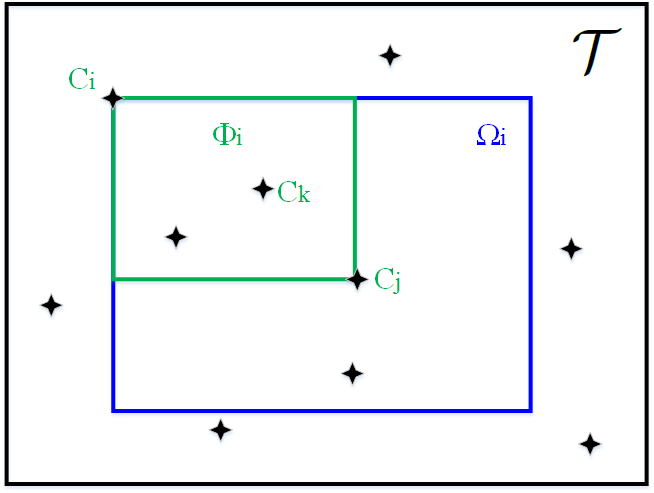
\includegraphics[width=2in,height=1.3in]{figures/algorithm.png}
	\caption{Rectangle region search algorithms.}
	\label{fig:rectangle_region}
\end{figure}

From the above analysis, we can see that the convex hull detection algorithm is too complex to realize. The root of this complexity lies in that we need to enumerate all the subset of $2^{\mathcal{T}}$.
To simplify our problem, we assume that the absenteeism region is a rectangle. Hence, the problem is transformed as: Given city set $\mathcal{T}$, areas upper bound $A$, determine the rectangle area
 \begin{equation}
 \mathcal{R}_{min}=\argmin\limits_{R\in 2^\mathcal{T}, s(\mathcal{R})\leq A}\Gamma_1(\mathcal{R})
\end{equation}

The rectangle minimal absenteeism group detection algorithm is described in Algorithm~\ref{algo:rectangle}.

\begin{algorithm}[t]
	\centering
	\captionsetup{font=scriptsize}
	\caption{Rectangle approximate algorithm.}
	{\footnotesize \begin{algorithmic}[1]
			\STATE {\bf Input:} city set $\mathcal{T}$, score set $\alpha(\mathcal{T})$ and areas upper bound $A$.
			\STATE {\bf Output:} rectangle $\mathcal{R}_{min}$ with lowest absenteeism score.
			\FORALL {each $c_i\in \mathcal{T}$}
			\STATE {assume $c_i$ as the most left-top point}	
			\STATE {select set $\Omega_i=\{c_j\}$; $\forall c_j\in \Omega_i, s(\mathcal{R}(c_i,c_j))\leq A$}
			\FORALL {each $c_j\in \Omega_i$}
			\STATE {compute group absenteeism score $\Gamma(\mathcal{R}(c_i, c_j))$}
			\ENDFOR	
			\STATE compute $\Gamma_{c_i}=\argmin\Gamma(\mathcal{R}(c_i, c_j))$, 	$\forall c_j\in \Omega_i$
			\ENDFOR
			\STATE{compute the $\Gamma_{min}=\argmin\Gamma_{c_i}, \forall c_i\in \mathcal{T}$}
			\RETURN $\Gamma_{min}$ and  $\mathcal{R}_{min}$.
		\end{algorithmic}}
		\label{algo:rectangle}
	\end{algorithm}
	
	
	
\begin{enumerate}
  \item Firstly, for each node $c_i\in \mathcal{T}$, it finds out the node set $\Omega_i$, such that $\forall c_j \in \Omega_i, \mathcal{R}(c_i, c_j)\leq A$. This step means when we fix $c_i$ as the most left-top vertex, then identify all the qualified rectangles. This step time complexity is $O(N)$.
\item Secondly, for each node $c_j \in \Omega_i$, compute group absenteeism score $\Gamma(\mathcal{R}(c_i,c_j))$, and then compute the $\Gamma_{c_i}=min\Gamma(\mathcal{R}(c_i, c_j))$ for all $c_j\in \Omega_i$. This step's time complexity depends on the node numbers of $\Omega_i$, which is denoted as $|\Omega_i|$. Suppose that nodes are uniformly distributed, thus $|\Omega_i|$ is directly proportional to $A$. Thus, this step's time complexity can be expressed as A, which is constant.
  \item Lastly, it returns the minimal $\Gamma_{min}=\Gamma_{c_i}, \forall c_i\in \mathcal{T}$.
\end{enumerate}
From the analysis, the rectangle algorithm time complexity is $A*N*A*N*N = O(N^3)$, which is greatly reduced comparing with the brute force algorithm.
%Figure~\ref{fig:mCoornidate} shows the most rectangle absenteeism group on Sep 11, 2013, when we set $A=0.02$.




\subsection{Subgraph approach}
For explanation convenience, we define some mathematic notation firstly.
\begin{itemize}
 \item $\mathcal{T}^-$ represents cities in $\mathcal{T}$ with negative absenteeism score, and can be expressed as $\mathcal{T}^-=\{c_i\}; \forall c_i\in \mathcal{T}$ and $\alpha(c_i)< 0$.
    \item Given city $c_i$ and distance threshold $d_{th}$, $\xi(c_i)$ means the cities whose distance to $c_i$ is closer than $d_{th}$. $\xi(c_i)$ can be expressed as $\xi(c_i)=\{c_j\}; \forall c_j\in \mathcal{T}$ and $d(c_i,c_j)< d_{th}$.
\end{itemize}
Essentially, a city set $\mathcal{T}$ is equivalent with an complete graph $G$, and any two cities $c_i$, and $c_j$ in $G$ are connected with distance of $d(c_i,c_j)$. The city absenteeism scores are mixed by both positive and negative ones. However for most circumstances, we are only interested with the cities which have the negative absenteeism scores, and are physically close enough to each other. Thus, we can think city set $\mathcal{T}^-$ into an complete graph, and identify the optimal subgraph $P_{min}$ which has the minimal group score, while its diameter $d(P_{min})\leq d_{th}$.\\
Thus, the problem is transformed as: Given city set $\mathcal{T}^-$, distance threshold $d_{th}$, identify city set $P_{min}\in 2^\mathcal{T^-}$, such that

 \begin{equation}
 P_{min}=\argmin\limits_{P\in 2^\mathcal{T^-}, s(P)\leq A}\Gamma_2(P)
\end{equation}

\begin{algorithm}[h]
	\centering
	\captionsetup{font=scriptsize}
	\caption{Subgraph approximate algorithm.}
	{\footnotesize \begin{algorithmic}[1]
			\STATE {\bf Input:} city set $\mathcal{T}$, score set $\alpha(\mathcal{T})$ and $d_{th}$.
			\STATE {\bf Output:} Subgraph $P_{min}$ with lowest absenteeism score
			\STATE find out $\mathcal{T}^-$ and $\alpha(\mathcal{T}^-)$
			\FORALL {$c_i \in \mathcal{T^-}$}
			\STATE identify $c_i$'s neighbors $\xi(c_i)$
			\STATE compute $\Gamma(\xi(c_i))$ 	
			\ENDFOR
			\RETURN ${P_{min}}$  and $\xi(c_i)$
		\end{algorithmic}}
		\label{algo:Subgraph}
	\end{algorithm}
	

\begin{table*}[t] %!htp
	\renewcommand{\arraystretch}{1}
	\caption{\label{table:list_events} Detected absenteeism groups over all the South America countries}
	\scriptsize
	\centering
	%\begin{tabular}{ p{3.5cm} | p{3.2cm} |p{2.9cm} | p{2.9cm} | p{2.9cm}}
	\begin{tabular}{ p{0.4cm}|l|l| p{8cm}|l | l}
		\hline
		\textbf{No.} & \textbf{Date}& \textbf{Country}& \textbf{ Events} & \textbf{ Period}  &  \textbf{ Method}   \\ [1ex]
		\hline
        1& 2013-06-20 & Brazil & Brazilian Spring: Protests in over 100 cities, over 2 million people &one day& Subgraph, regional \\
        2& 2013-08-31 & Peru & Peru snow state of emergency extended to more regions & one day&regional \\
        3& 2013-09-03 & Venezuela & Power cut leaves much of Venezuela without electricity &one day& subgraph\\
		4& 2013-09-11 & Mexico & Mexico teachers protest against education reform in 17 cities &15:00-15:30 &Subgraph \\
        5& 2013-10-17 & Colombia & Floods, particularly heavy rains affecting south-west of Colombia & one day& regional \\
        6& 2013-12-24 & Brazil & Floods, more than 50,000 people are forced to flee their homes&one day& subgraph, regional \\
        7& 2013-12-30 & Argentina &  Power supply disrupted in heatwave in Buenos Aires, Argentina. &one day&subgraph\\
        8& 2014-01-09 & Bolivia & Floods & one day&regional, subgraph \\
        9& 2014-01-31 & Chile & Chile`S IPSA stock index hit lows not seen in over 4 years & one day&regional\\
        10& 2014-02-12 & Bolivia & Heavy rain caused floods and landslides in several parts of Bolivia &one day& regional, subgraph\\
        11 & 2014-02-13 & Argentina & Heavy rain and landslides & one day&subgraph\\
        %12& 2014-02-19 & Venezuela & Earthquake M5.5, 49000 people exposed to strong shaking &6:30AM &regional \\
        12& 2014-02-27 & Venezuela & Social unrest & one day&subgraph, regional \\
        %14& 2014-03-15 & Peru& Earthquake shaking up to Very Strong for 45 000 people &17:30PM &subgraph \\
        13& 2014-03-24 & Chile & People in Chile on edge over unusual string of 300 tremors &one day&subgraph\\
        %16& 2014-03-31 & Chile & Earthquake M5.6 &7:30AM &subgraph\\
        14& 2014-04-01 & Chile &  M8.2 earthquake struck off the coast of Chile, epicenter is Iquique & 20:45-20:50 &subgraph \\
        15& 2014-05-01 &Central America& Labor Day, national holiday &one day &Subgraph, regional \\
        16& 2014-05-16 & Brazil & Anti-World Cup protests in 12 cities of Brazil &one day& subgraph, regional \\
        17& 2014-05-21 & Brazil & Bus strike paralyzes Brazil's biggest city as World Cup looms &9:30-10:00& regional\\				
		\hline
	\end{tabular}
\end{table*}



An obvious brute force algorithm would be enumerate all the possible $P\in 2^\mathcal{T^-}$, thus the complexity would be $2^{N^-}$. Usually $N^-$ is larger than 100, which makes the brute force algorithm uncritical. Algorithm~\ref{algo:Subgraph} gives out an approximate algorithm with $O(N^2)$ running time complexity.
\begin{enumerate}
  \item Firstly, it determines the subset $\mathcal{T}^-$ since we only concern the negative absenteeism cities.
  \item Secondly, for each node $c_j \in \mathcal{T}^-$, it identifies neighbor $\xi(c_i)$ and $\Gamma(\xi(c_i))$. In $\xi(c_i)$,  each node's distance to $c_i$ is smaller than $d_{th}$. $\forall c_{j1}, c_{j2}\in \xi(c_i$ and $c_{j2}$ , $d(c_{j1}, c_{j2})\leq d(c_{j1}, c_i)+d(c_{j2}, c_i)\leq 2d_{th}$. Thus, this approximate algorithm can guarantee the diameter of $P_{min}$ is less than $2d_{th}$. Evidently, this step's time complexity is linear because it need to enumerate $c_i$ to all other node in $\mathcal{T}^-$.
  \item Lastly, it returns the minimal $\Gamma_{min}=\Gamma_{c_i}, \forall c_i\in \mathcal{T}$.
\end{enumerate}




% % % % % % % % % % % % % the end % % % % % % % % % % % % %
